\documentclass{article}
\usepackage{blindtext}
\usepackage[a4paper, total={6in, 8in}]{geometry}

\usepackage{wrapfig}
\usepackage{graphicx}
\usepackage{mathtext}
\usepackage{amsmath}
\usepackage{siunitx} % Required for alignment
\usepackage{subfigure}
\usepackage{multirow}
\usepackage{rotating}
\usepackage[T1,T2A]{fontenc}
\usepackage[russian]{babel}
\usepackage{caption}


\graphicspath{{pictures/}}


\title{\begin{center}Лабораторная работа №2.2.1\end{center}
Исследование взаимной диффузии газов}
\author{Гёлецян А.Г.}
\date{\today}

\begin{document}
    \pagenumbering{gobble}
    \maketitle
    \newpage
    \pagenumbering{arabic}

\textbf{Цель работы:} 1) регистрация зависимости концентрации гелия в воздухе от времени с помощью датчиков теплопроводности при разных начальных давлениях смеси газов; 2) определение коэффициента диффузии по результатам измерений.

\textbf{В работе используются:} измерительная установка; форвакуумный насос; балон с газом  (гелий); манометр; источник питания; магазин сопротивлений; гальванометр; секундомер.


\section{Теоретическая часть}
    \textit{Диффузией}  называют самопроизвольное взаимное проникновение веществ друг в друга происходящее вследствие хаотичного теплового движения молекул. При перемешивании молекул разного сорта говорят о взаимной (или концентрационной) диффузии. В системе, состоящей из двух компонентов a и b (бинарная смесь), плотности потоков частиц в результате взаимной диффузии определяются законом Фика:
    \begin{equation}
        j_a = -D \frac{\partial n_a}{\partial x}, \, j_b = -D \frac{\partial n_b}{\partial x},
    \end{equation}
    где $D$ — \textit{коэффициент взаимной диффузии компонентов}. Знак <<минус>> отражает тот факт, что диффузия идёт в направлении выравнивания концентраций. Равновесие достигается при равномерном распределении вещества по объёму.

    В данной работе исследуется взаимная диффузия гелия и воздуха. Отметим, что давление и температура в системе предполагаются неизменным: $P_0 = (n_{He}+n_{Air})kT = const$, где $n_{He}$  и $n_{Air}$ -- концентрации диффундирующих газов. Поэтому для любых изменений концентраций справедливо $\Delta n_{Air} = -\Delta n_{He}$. Следовательно, достаточно ограничиться описанием диффузии одного из компонентов, например гелия.

    Приведём теоретическую оценку для коэффициента диффузии. В работе концентрация гелия, как правило, мала ($n_{He} \ll n_{Air}$). Кроме того, атомы гелия легче молекул, составляющих воздух ($m_{He} \ll m_{N_2}, m_{O_2}$), значит их средняя тепловая скорость велика по сравнению с остальными частицами. Поэтому перемешивание газов в работе можно приближенно описывать как диффузию примеси лёгких частиц He на практически стационарном фоне воздуха. Коэффициент диффузии в таком приближении равен
    \begin{equation}
        \label{D}
        D = \frac{1}{3} \lambda \langle v \rangle,
    \end{equation}
    где $\lambda = \frac{1}{n\sigma}$ -- длина свободного пробега диффундирующих частиц; $\langle v \rangle = \sqrt{\frac{8kT}{\pi m}}$ -- их средняя тепловая скорость.

    Предпологая, что процесс диффузии будет квазиостационарным, можно показать, что разность концентраций будет убывать по экспоненциальному закону
    \begin{equation}
        \label{Delta_n}
        \Delta n = \Delta n_0 e^{-t / \tau},
    \end{equation}
    где $\tau$ -- характерное время выравнивания концентраций между сосудами, определяемое следующей формулой
    \begin{equation}
        \label{Tau}
        \tau = \frac{1}{D} \frac{V_1V_2}{V_1 + V_2} \frac{L}{S}.
    \end{equation}

\section{Модель эксперимента}
    Для   исследования   взаимной диффузии газов и измерения коэффициента взаимной диффузии  $D$  используется  два сосуда  объёмами  $V_1$ и $V_2$ ($V_1 \approx V_2$), соединенные трубкой длины $L$ и сечения  $S$. Предполагается, что сосуды заполнены смесью двух газов при одинаковом давлении, но с различной концентрацией компонентов. Вследствие взаимной диффузии, проходящей в   соединительной трубке, концентрации компонентов в сосудах с течением времени выравниваются.

    Для измерения разности  концентраций  в установке применяются датчики теплопроводности. При этом используется тот факт, что теплопроводность смеси $\kappa$ зависит от её состава. В общем случае   зависимость  $\kappa (n)$  довольно   сложна,   однако   при   малой   разности  $\Delta n$ концентраций в сосудах можно ожидать, что разность теплопроводностей будет изменяться прямо пропорционально $\Delta n:$
    \begin{equation*}
        \Delta \kappa = \kappa (n_2) - \kappa (n_1) \approx const \cdot \Delta n.
    \end{equation*}

    Эксперименты показывают, что если доля примеси гелия составляет менее 15\%, отклонение от линейной зависимости не превышает 0,5\%, что для наших целей вполне достаточно.


    При заданной мощности нагревания приращение температуры  проволочки и, следовательно, приращение её сопротивления пропорциональны теплопроводности газа. Для измерения сопротивлений используется мостовая схема, позволяющая определять разность показаний датчиков с высокой точностью. Мост балансируется при заполнении сосудов (и датчиков) одной и той же смесью. При заполнении сосудов смесями различного состава возникает «разбаланc» моста. При незначительном различии в составах смесей показания гальванометра, подсоединённого к диагонали моста, будут пропорциональны разности концентраций примеси: $U\propto\Delta \kappa \propto \Delta n$. В процессе диффузии разность концентраций убывает по закону~(\ref{Delta_n}), и значит по тому же закону изменяются во времени показания гальванометра
    \begin{equation}
        U = U_0 \, e^{-t / \tau},
    \end{equation}
    где $U_0$ -- показание в начальный момент времени. Измеряя экспериментально зависимость $U(t)$, можно получить характерное время процесса $\tau$, откуда по формуле~(\ref{Tau}) определить коэффициент диффузии $D$.

    \section{Ход работы}
    Для нашей установки имеем
    \[V_1=V_2=(775 \pm 10)см^3\]
    \[\frac{L}{S} = (5.3 \pm 0.1)см^{-1}\]

    Для удобства сразу подсчитаем известную часть в правой части уравнения (4)
    \[\frac{V_1V_2}{V_1 + V_2} \frac{L}{S} = (2050 \pm 60)см^2\]

    По циклу накачка воздуха - балансировка - откачка - накачка гелием и воздухом - выравнивание давления - измерение проводим 5 измерении при различных рабочих давлениях. Результаты измерении приведены на графике (2). Согласно формуле (5)
    \[ln(U) = -\frac{t}{\tau} + C\]
    Построим логарифмический график (3) и найдем $\tau$ используя наклон аппроксимированной прямой. Данные для времен релаксации приведены в таблице (1).


    \begin{table}[h!]
        \vspace{5pt}
        \begin{center}
        \begin{tabular}{|l|rr|}
        \hline
        $P_{раб}$ & $\tau$ & $\Delta \tau$ \\
        торр & с & с\\
        \hline
        41 & 212.06 & 0.14 \\
        80 & 346.6 & 0.4 \\
        120 & 518.7 & 0.9 \\
        160 & 665.3 & 3.0 \\
        200 & 826.7 & 4.0 \\
        \hline
        \end{tabular}

        \caption{Времена релаксации в зависимости от давления.}
        \label{data}
        \end{center}
    \end{table}

    Посчитаем коэффиценты диффузии и их ошибки по формуле (4).

    \begin{table}[h!]
        \vspace{5pt}
        \begin{center}
        \begin{tabular}{|l|rr|}
        \hline
        $P_{раб}$ & $D$ & $\Delta D$ \\
        торр & $см^2с^{-1}$ & $см^2с^{-1}$\\
        \hline
        41 & 9.67 & 0.28 \\
        80 & 5.92 & 0.17 \\
        120 & 3.95 & 0.12 \\
        160 & 3.08 & 0.09 \\
        200 & 2.48 & 0.07 \\
        \hline
        \end{tabular}

        \caption{Коэффиценты диффузии в зависимости от давления.}
        \label{data}
        \end{center}
    \end{table}

    Согласно формуле (2) величины $D$ и $1/P$ связаны соотношением
    \begin{equation}
    D = \frac{kT}{3\sigma} \sqrt{\frac{8RT}{\pi \mu_{He}}}  \frac{1}{P}
    \end{equation}

    Построим график (1) зависимости $D$ от $1/P$ чтобы проверить это. Как видим, линейная зависимость не идеальная, но все равно зависимость похоже на линейную. Если считать зависимость линейной и сделать аппроксимацию, получим

    \begin{equation}
        \frac{kT}{3\sigma} \sqrt{\frac{8RT}{\pi \mu_{He}}} = (370 \pm 40) см^2торр/с = (4.93 \pm 0.53)\frac{Дж}{м^2}\frac{м}{с}
    \end{equation}

    Подставляем комнатную температуру $T = 22 ^\circ C$ и получаем

    \begin{equation}
        \sigma = (3.45 \pm 0.37) 10^{-19}м^2
    \end{equation}


    \begin{figure}[h]
        \center{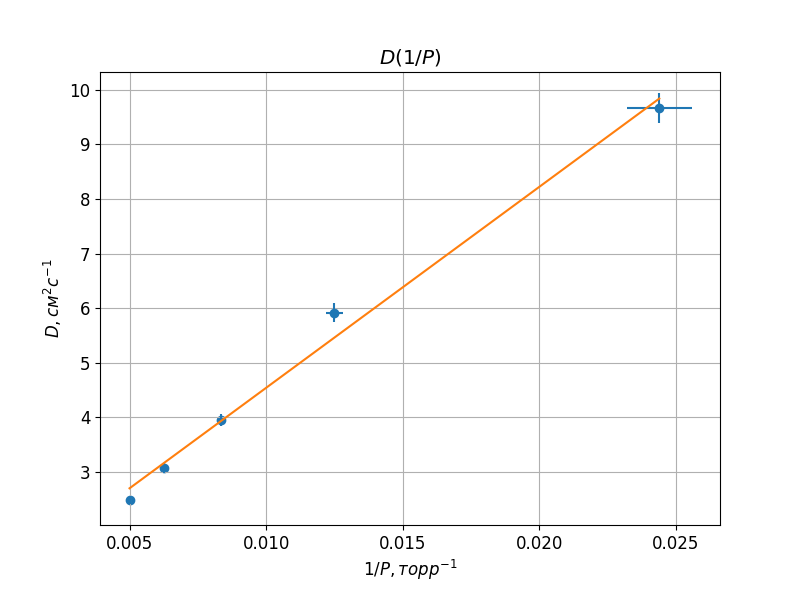
\includegraphics[width=\textwidth]{D}}
        \caption{Зависимость $D(1/P)$.}
        \label{ustanovka}
    \end{figure}

    \newpage
    \section{Выводы}
    Нами было получено соотношение
    \[D = (370 \pm 40)\frac{см^2}{с} \frac{1торр}{P}\]
    При атмосферном давлении $P_0=760 торр$ наше соотношение выдает
    \[D_0 = (0.49 \pm 0.05)\frac{см^2}{с}\]

    тыбличные данные указывают на значение
    \[D_{табл} = 0.62\frac{см^2}{с}\]
    Относительная ошибка нашего результата $\varepsilon = 20\%$.
    \newpage
    \begin{sidewaysfigure}[h!]
        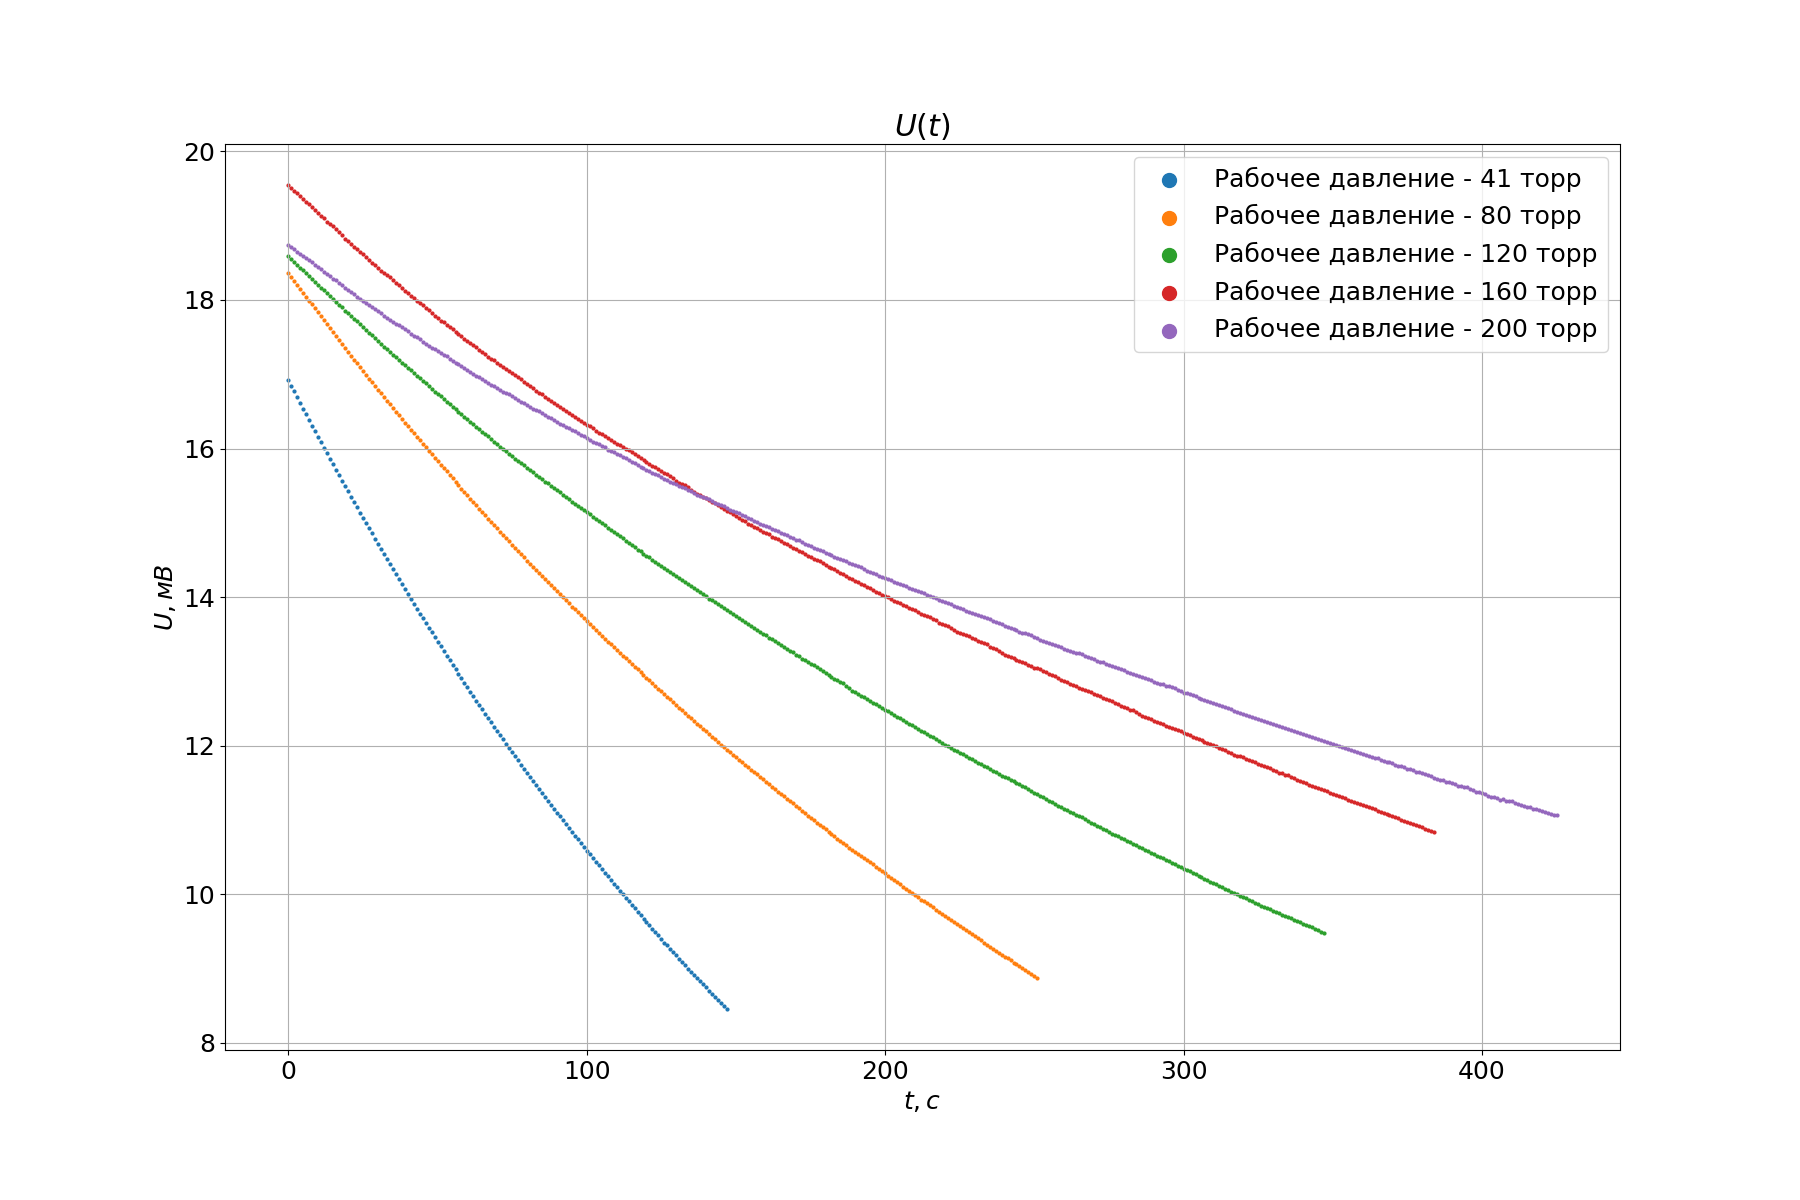
\includegraphics[width=1.2\textwidth]{U(t)}
        \label{U}
        \caption{Зависимость $U(t)$.}
    \end{sidewaysfigure}
    \newpage
    \begin{sidewaysfigure}[h!]
        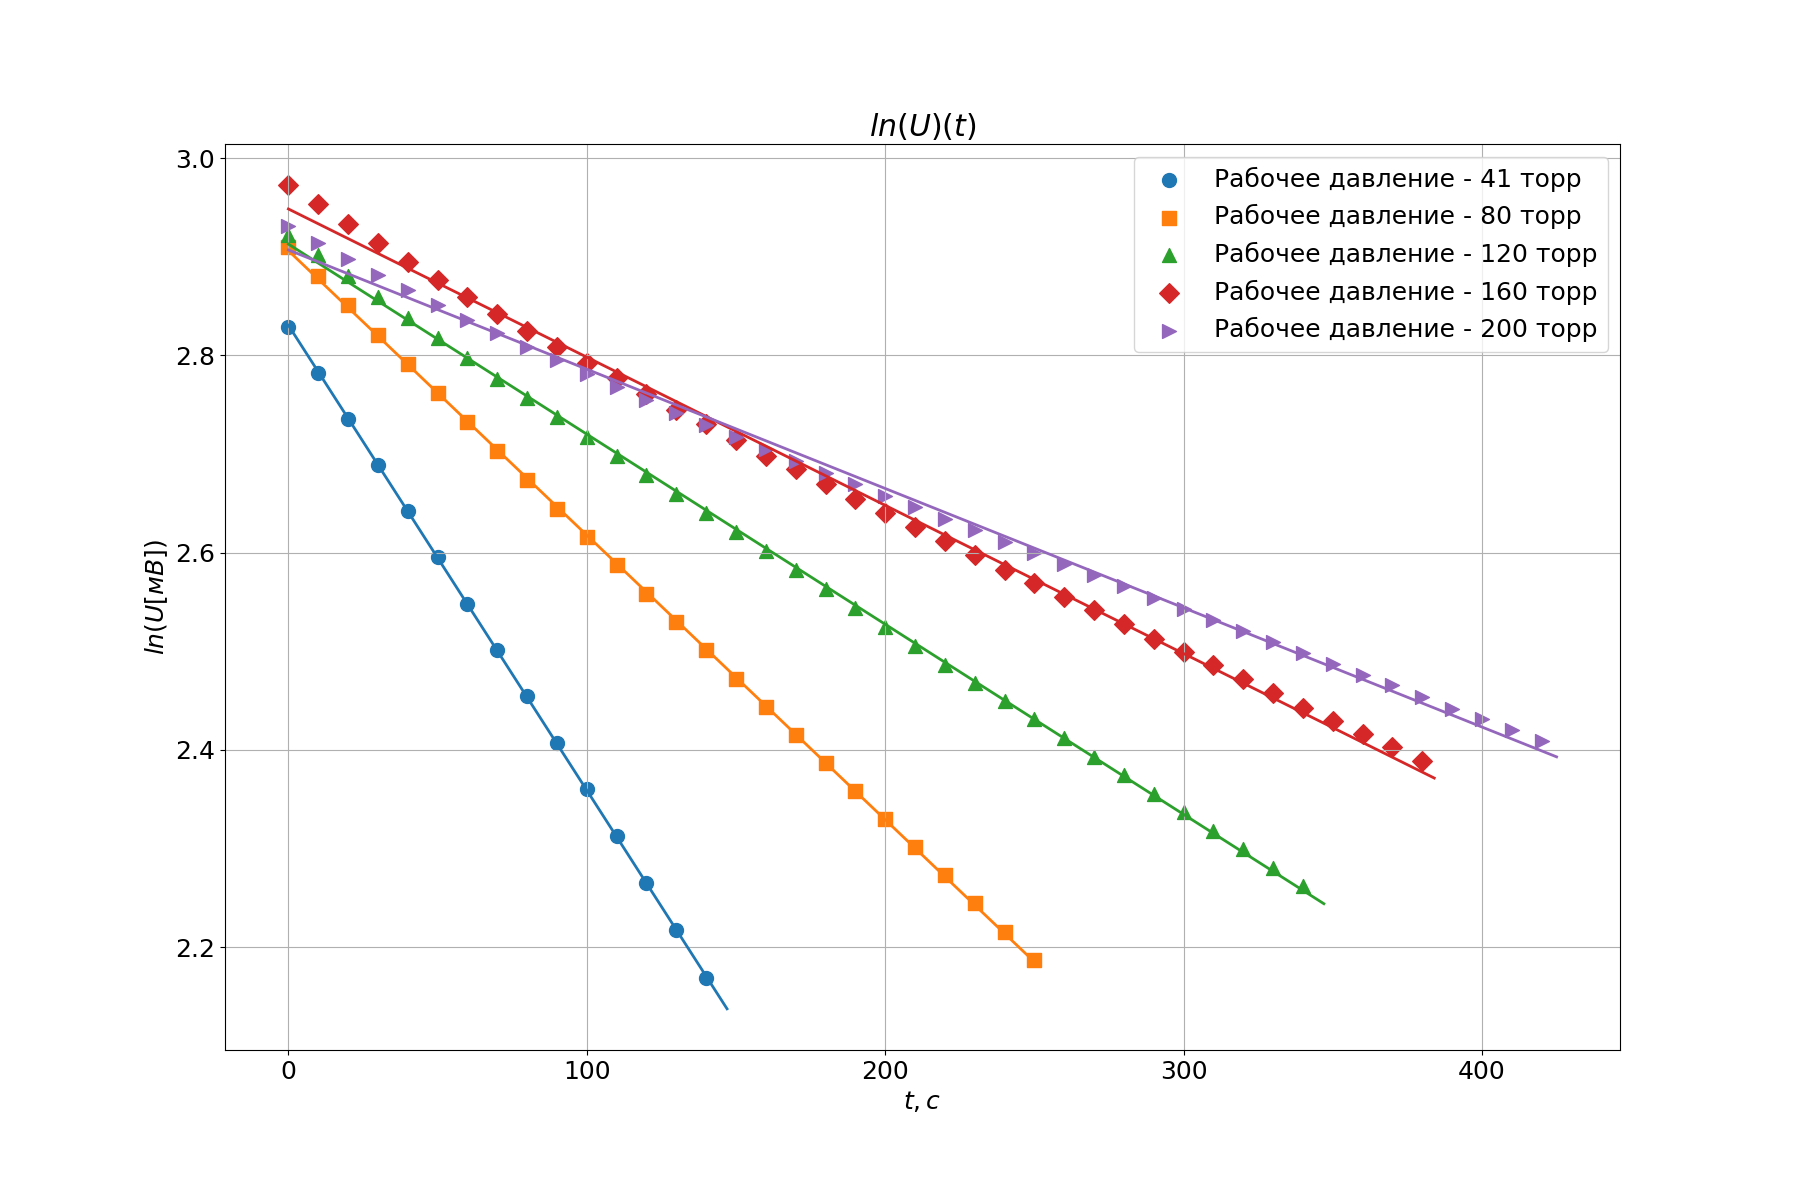
\includegraphics[width=1.2\textwidth]{lnU(t)_mnk}
        \label{lnU}
        \caption{Зависимость $ln(U)(t)$.}
    \end{sidewaysfigure}
    \newpage
\end{document}



